% Chapter 15: Security Protocol Verification with Tamarin
% Sources: Course 89, L27-L28

\chapter{Security Protocol Verification with Tamarin}
\label{ch:tamarin}

\aside{Chapter~\ref{ch:ctl-symbolic} reasoned about sets of states.  Security
protocols need a different state model: not a control bit-vector, but a live
multiset of facts describing who knows what, which role instance is active,
and which messages have moved across the network.}

The last chapter ended with symbolic verification over Boolean state sets.
Tamarin moves that symbolic idea into a message-passing world.  Instead of a
transition relation over bits, we use multiset rewriting over facts; instead
of model states, we track protocol roles, network messages, and attacker
knowledge; instead of a single execution graph, we reason about traces
generated by rule instances.  The point is the same: compress an enormous
search space into a representation we can still manipulate mechanically.  The
difference is the object being represented.

Tamarin is not just a theoretical toy. It has had massive real-world impact. During the standardisation of the 5G mobile protocol, researchers used Tamarin to formally analyze the authentication handshakes. They discovered critical flaws that would have allowed attackers to break user anonymity and track mobile devices as they moved between antennas. The standard was subsequently patched based on Tamarin's proofs. It has also been used to find flaws in TLS 1.3 draft specifications.

The chapter follows the core ideas that recur in the Tamarin lecture block.
We begin with the intuition behind protocol verification and the Dolev-Yao
attacker model.  Then we build the syntax and semantics of multiset rewriting
from the ground up: terms, facts, fresh names, and rewrite rules.  After that
we shift from individual rules to protocol roles and traces, which is where a
local step description becomes a global execution history.  The closing section
shows how Tamarin states properties over traces and searches for proofs or
counterexamples.

\begin{chapteropening}
\textbf{Where we are.}  Symbolic model checking compressed large Boolean state
spaces into formulas and decision diagrams.  Security protocols need the same
kind of compression, but their states are not fixed bit-vectors.

\textbf{What this chapter adds.}  Tamarin represents protocol executions with
terms, facts, multiset rewrite rules, and traces.  This lets us reason about
fresh names, adversary knowledge, role instances, and long-lived secrets in a
single symbolic framework.

\textbf{Where it leads.}  The chapter closes the notes by showing how the
verification ideas developed for automata and transition systems become a
tool-supported workflow for real security protocols.

\textbf{Chapter map.}
\begin{itemize}[nosep]
  \item \Cref{sec:tamarin-intuition} moves from state machines to protocol
        histories.
  \item \Cref{sec:tamarin-msr} defines terms, facts, and multiset rewriting
        rules.
  \item \Cref{sec:tamarin-roles-traces} connects local protocol roles to
        global traces.
  \item \Cref{sec:tamarin-unification} explains equational theories and
        unification.
  \item \Cref{sec:tamarin-properties} states secrecy, authentication, and
        trace properties.
  \item \Cref{sec:tamarin-summary} distils the modelling discipline.
\end{itemize}
\end{chapteropening}

% =======================================================================
\section{From State Machines to Protocol Histories}
% Sources: Course 89, L27
\label{sec:tamarin-intuition}

Security protocols are not ordinary transition systems.  A controller model
usually has a small, fixed set of control locations and a neat transition
graph.  A protocol model has messages, nonces, long-term keys, sessions,
replays, and an adversary who can store, forward, combine, and fabricate
messages.  The interesting question is therefore not just ``which control
state comes next?'' but ``which facts are currently in scope, which messages
can be derived, and which role instances can continue?''

\begin{intermezzo}{Why protocol verification looks stateful}
The state of a protocol run is not only the local control state of the honest
participants.  It also includes the messages in flight, the facts the
adversary has learned, and the fresh values that were created earlier in the
run.  Tamarin keeps all of that in a single symbolic object: a multiset of
facts.
\end{intermezzo}

The standard abstraction behind Tamarin is the Dolev-Yao model.  Messages are
symbolic terms, not bitstrings.  Cryptography is idealised by equations and by
the intruder's deduction power: if a message is sent on the network, the
attacker can see it; if the attacker can derive a message from what it knows,
it can send that message back on the network.  Honest participants do not get
special protection from the model.  They survive only if the protocol rules
force the attacker to miss a crucial piece of information.

That model is deliberately austere, but it is exactly what we need for
protocol analysis.  It lets us describe the protocol once, then quantify over
all possible attacker behaviours.  In the lecture material, this is the move
from ``one run we can simulate'' to ``all runs we must inspect''.

\begin{figure}[ht]
  \centering
  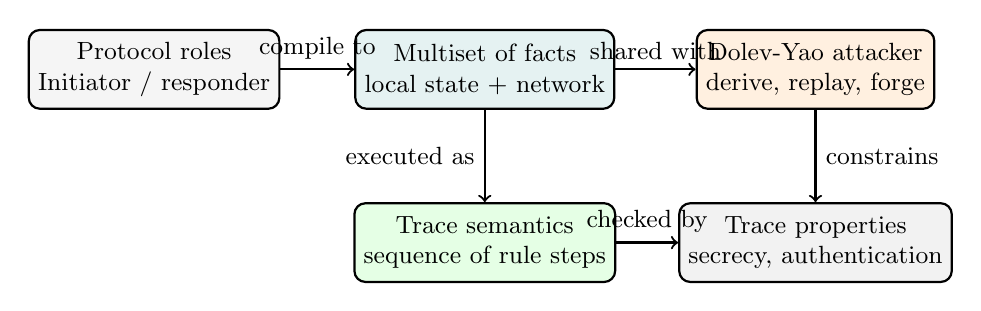
\begin{tikzpicture}[
      box/.style={draw, rounded corners, minimum width=3.0cm,
                  minimum height=1.0cm, align=center, font=\small, thick},
      arr/.style={->, thick}
    ]
    \node[box, fill=gray!8]   (roles) at (0,0) {Protocol roles\\Initiator / responder};
    \node[box, fill=teal!10]  (facts)  at (4.2,0) {Multiset of facts\\local state + network};
    \node[box, fill=orange!12] (adv)   at (8.4,0) {Dolev-Yao attacker\\derive, replay, forge};
    \node[box, fill=green!10] (trace)  at (4.2,-2.2) {Trace semantics\\sequence of rule steps};
    \node[box, fill=gray!10]  (props)  at (8.4,-2.2) {Trace properties\\secrecy, authentication};

    \draw[arr] (roles) -- node[above, font=\small] {compile to} (facts);
    \draw[arr] (facts) -- node[above, font=\small] {shared with} (adv);
    \draw[arr] (facts) -- node[left, font=\small] {executed as} (trace);
    \draw[arr] (trace) -- node[above, font=\small] {checked by} (props);
    \draw[arr] (adv) -- node[right, font=\small] {constrains} (props);
  \end{tikzpicture}
  \caption{Tamarin keeps the protocol, the attacker, and the property in one
           symbolic picture.  Roles generate facts, facts generate traces, and
           traces are the object on which properties are checked.}
  \label{fig:tamarin-overview}
\end{figure}

\subsection{Case study: Designing a secure key exchange}

To understand why security protocol verification requires specialized tools, we trace the step-by-step design of a protocol to establish a shared session key $K_{AB}$ between Alice ($A$) and Bob ($B$) with the help of a trusted server $S$. This case study highlights how easily subtle vulnerabilities can slip into seemingly simple designs.

\subsubsection{Attempt 1: Plaintext exchange}
We assume Alice wants to communicate with Bob. She contacts the server, requesting a session key:
\[
  A \to S : A, B
\]
The server generates a fresh session key $K_{AB}$ and sends it to Alice:
\[
  S \to A : K_{AB}
\]
Alice then forwards the key to Bob:
\[
  A \to B : K_{AB}
\]
\textbf{Vulnerability (Eavesdropping)}: Since the network is insecure and controlled by the Dolev-Yao attacker, the intruder can read all messages in transit. The attacker learns $K_{AB}$ immediately from the server's reply or from Alice's forward. Secrecy is completely lost.

\subsubsection{Attempt 2: Encrypted key distribution (no identities)}
To protect the session key, we strengthen our assumptions. We assume that Alice shares a long-term secret symmetric key $K_{AS}$ with the server, and Bob shares a key $K_{BS}$ with the server. Now, the server can encrypt the session key:
\begin{align*}
  A \to S &: A, B \\
  S \to A &: \{K_{AB}\}_{K_{AS}}, \, \{K_{AB}\}_{K_{BS}} \\
  A \to B &: \{K_{AB}\}_{K_{BS}}
\end{align*}
Alice decrypts $\{K_{AB}\}_{K_{AS}}$ to learn the session key, and forwards the second encrypted package to Bob. Bob decrypts it using $K_{BS}$ to learn $K_{AB}$.

\textbf{Vulnerability (Man-in-the-Middle)}: An intruder $I$, who is a registered user of the system and shares a key $K_{IS}$ with the server, can intercept Alice's request and launch a Man-in-the-Middle (MITM) attack:
\begin{enumerate}
  \item Alice initiates communication with Bob: $A \to S : A, B$.
  \item The intruder intercepts this message and tampers with Bob's identity, replacing it with his own: $I(A) \to S : A, I$.
  \item The server thinks Alice wants to communicate with the intruder. It generates a session key $K_{AI}$ and replies:
  \[
    S \to A : \{K_{AI}\}_{K_{AS}}, \, \{K_{AI}\}_{K_{IS}}
  \]
  \item The intruder intercepts this reply. Since he knows $K_{IS}$, he decrypts $\{K_{AI}\}_{K_{IS}}$ and learns $K_{AI}$.
  \item The intruder forwards $\{K_{AI}\}_{K_{AS}}$ to Alice.
  \item Alice decrypts it. Because the encrypted payload does not contain the identity of her intended partner, she assumes that $K_{AI}$ is the session key shared with Bob.
\end{enumerate}
Alice now encrypts her messages for Bob using $K_{AI}$. The intruder intercepts them, decrypts them (since he knows $K_{AI}$), and can read or modify them before optionally re-encrypting them and forwarding them to Bob.

\subsubsection{Attempt 3: Encrypted key with identities}
To prevent the MITM attack, the server must explicitly bind the session key to the identities of the intended participants inside the encrypted payloads:
\begin{align*}
  A \to S &: A, B \\
  S \to A &: \{K_{AB}, B\}_{K_{AS}}, \, \{K_{AB}, A\}_{K_{BS}} \\
  A \to B &: \{K_{AB}, A\}_{K_{BS}}
\end{align*}
If the intruder attempts the same tampering ($I(A) \to S : A, I$), the server replies with $\{K_{AI}, I\}_{K_{AS}}$. When Alice decrypts this, she sees that the key is bound to the intruder's identity $I$ rather than Bob's, detects the discrepancy, and aborts the protocol.

\textbf{Vulnerability (Replay attack)}: Suppose Alice and Bob successfully run the protocol and establish a session key $K_{AB}$. The intruder eavesdrops and stores the message $A \to B : \{K_{AB}, A\}_{K_{BS}}$ on his hard drive.

Now, imagine that five years later, the session key $K_{AB}$ is compromised (e.g., through brute force or cryptanalysis). The intruder can now spoof Alice and replay the old encrypted message to Bob:
\[
  I(A) \to B : \{K_{AB}, A\}_{K_{BS}}
\]
Bob decrypts the message, sees that it is a valid ciphertext encrypted by the server containing Alice's identity, and accepts $K_{AB}$ as a fresh, secure session key. The intruder can now impersonate Alice to Bob or decrypt Bob's messages. This attack succeeds because Bob has no way of verifying the \emph{freshness} of the message, highlighting the need for nonces or timestamps in security protocol design.

\medskip\noindent
\textbf{The bridge from Chapter~\ref{ch:ctl-symbolic}.}  Symbolic model
checking represented sets of states by Boolean formulas.  Tamarin represents
reachable protocol situations by multisets of facts and searches the induced
trace space.  The level of abstraction is comparable; the underlying object
is simply different.


% =======================================================================
\section{Multiset Rewriting: Terms, Facts, and Rules}
% Sources: Course 89, L27
\label{sec:tamarin-msr}

\subsection{Terms}

At the base of the formalism are symbolic messages, which Tamarin calls
\emph{terms}.  We stay in the free term algebra for the core presentation.

\begin{definition}[Terms]
\label{def:tamarin-terms}
Let $\mathcal{N}$ be a set of names, $\mathcal{V}$ a set of variables, and
$\mathcal{F}$ a set of function symbols with fixed arities.  The set of
terms is generated by
\[
  t ::= n \mid x \mid f(t_1,\dots,t_k)
\]
where $n \in \mathcal{N}$, $x \in \mathcal{V}$, and $f \in \mathcal{F}$ has
arity $k$.  Fresh names are usually written with a tilde, such as $\tilde n$,
to indicate that they are generated during a protocol run.
\end{definition}

\medskip\noindent
\textbf{Idealized Cryptography and Probabilities.} In reality, when a protocol generates a 256-bit random nonce $\tilde n$, an attacker has a tiny, non-zero probability of guessing it correctly. Tamarin explicitly idealizes this. Fresh values are modeled symbolically so that they absolutely \emph{cannot} be guessed by the attacker. The tiny cryptographic probability is abstracted into a rigorous zero, allowing the tool to focus entirely on logical flaws rather than statistical ones.

Terms are the symbolic payloads of the protocol.  A nonce, a key, a pair of
values, or an encrypted message are all just terms.  The point is not that
the model knows how to perform real cryptography.  The point is that the
model can talk about who created which symbolic value and who later saw it.

\begin{example}[A message term]
If an initiator sends its identity together with a fresh nonce, the network
message can be represented by the term
\[
  \langle A,\tilde n\rangle.
\]
If the protocol later nests this value inside a larger structure, the term
tree records that structure explicitly.  There is no hidden state inside the
message.  Every piece of information that matters is present in the term.
\end{example}

\subsection{Facts}

Facts are the protocol state.  They are the resources, memories, and events
that a rule can consume or produce.

\begin{definition}[Facts]
\label{def:tamarin-facts}
A fact is an atom of the form $F(t_1,\dots,t_k)$, where $F$ is a predicate
symbol and the $t_i$ are terms.  Facts may be linear or persistent.  A
persistent fact is written with a leading bang, as in $!F(t_1,\dots,t_k)$.
\end{definition}

Linear facts are consumed when a rule fires.  Persistent facts remain
available after use.  This distinction is one of the most useful parts of the
formalism:
\begin{itemize}
  \item linear facts model one-shot resources, local control states, and
        ephemeral protocol state;
  \item persistent facts model long-term keys, static configuration, or any
        fact that should survive across multiple rule applications.
\end{itemize}

The most common special facts are the network facts:
\begin{itemize}
  \item $\mathsf{Out}(m)$ publishes a message to the network;
  \item $\mathsf{In}(m)$ consumes a message from the network.
\end{itemize}
The adversary sees every $\mathsf{Out}(m)$ and may later supply any message
that can be built from its current knowledge.  In other words, the attacker is
not an extra agent bolted onto the model afterwards.  It is part of the
semantics of how network facts are interpreted.

\subsection{Rewrite rules}

Protocols evolve by rewriting one multiset of facts into another.

\begin{definition}[Multiset rewriting rule]
\label{def:tamarin-rule}
A rewrite rule has the shape
\[
  L \; \xrightarrow{\;A\;} \; R
\]
where $L$ and $R$ are multisets of facts and $A$ is a multiset of action
facts.  Informally, $L$ is the rule's premise, $R$ is its conclusion, and $A$
records the observable events generated by the step.
\end{definition}

An instance of a rule is obtained by choosing a substitution $\sigma$ for the
variables in the rule so that the left-hand side matches a submultiset of the
current state.  Then the matching facts are consumed, the right-hand side is
added, and the action facts are appended to the trace.  Fresh names are
created at the moment the rule fires, so a rule using a fresh variable really
does create a new symbolic value.

\begin{definition}[One rewriting step]
\label{def:tamarin-step}
Let $M$ be a multiset of facts and let $L \xrightarrow{A} R$ be a rule.
If there exists a substitution $\sigma$ such that $L\sigma \subseteq M$,
then one step of rewriting produces
\[
  M' = (M \setminus L\sigma) \uplus R\sigma.
\]
The corresponding action facts $A\sigma$ are recorded in the trace.
\end{definition}

\medskip\noindent
\textbf{Intuition: Sticky notes on a fridge.}  Imagine a large whiteboard or a fridge. A multiset of facts is just a collection of sticky notes placed on the fridge. When a rule fires, you remove specific sticky notes (linear facts) and slap on new ones. Persistent facts are like sticky notes glued to the fridge permanently. The trace is a ledger remembering every sticky note you ever moved.

Why do we need a \emph{multi}set instead of a normal set? Because a single protocol can be instantiated multiple times concurrently. If Alice starts two simultaneous sessions, there will be two identical \texttt{start\_Alice} sticky notes on the fridge. Set semantics would collapse them into one, breaking the ability to track independent parallel sessions. Multisets allow multiple identical sticky notes.

\begin{figure}[ht]
  \centering
  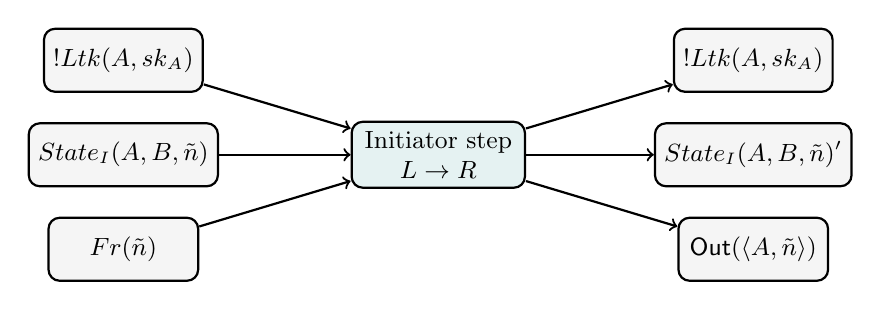
\begin{tikzpicture}[
      fact/.style={draw, rounded corners, minimum width=1.9cm,
                   minimum height=0.8cm, align=center, font=\small, thick,
                   fill=gray!8},
      rule/.style={draw, rounded corners, minimum width=2.2cm,
                   minimum height=0.8cm, align=center, font=\small, thick,
                   fill=teal!10},
      arr/.style={->, thick}
    ]
    \node[fact] (left1) at (0,1.2) {$!Ltk(A,sk_A)$};
    \node[fact] (left2) at (0,0) {$State_I(A,B,\tilde n)$};
    \node[fact] (left3) at (0,-1.2) {$Fr(\tilde n)$};

    \node[rule] (r) at (4,0) {Initiator step\\$L \to R$};

    \node[fact] (right1) at (8,1.2) {$!Ltk(A,sk_A)$};
    \node[fact] (right2) at (8,0) {$State_I(A,B,\tilde n)'$};
    \node[fact] (right3) at (8,-1.2) {$\mathsf{Out}(\langle A,\tilde n\rangle)$};

    \draw[arr] (left1) -- (r);
    \draw[arr] (left2) -- (r);
    \draw[arr] (left3) -- (r);
    \draw[arr] (r) -- (right1);
    \draw[arr] (r) -- (right2);
    \draw[arr] (r) -- (right3);
  \end{tikzpicture}
  \caption{A rewrite rule consumes linear facts, preserves persistent facts,
           and emits new facts and action facts.  The trace stores the rule
           application even when the consumed facts disappear from the state.}
  \label{fig:tamarin-rewrite}
\end{figure}

\subsection{A concrete toy protocol}

The simplest way to see the machinery is to write down a tiny handshake.
The protocol is intentionally small; the goal is to show the shape of the
rules, not to claim cryptographic strength.

\begin{lstlisting}
rule Initiate:
  [ Fr(~na), !Ltk(A, skA) ]
  --[ Begin(A, B, ~na) ]->
  [ StateI(A, B, ~na), Out(<A, ~na>) ]

rule Respond:
  [ In(<A, na>), Fr(~nb), !Ltk(B, skB) ]
  --[ End(B, A, na, ~nb) ]->
  [ StateR(B, A, na, ~nb), Out(<na, ~nb>) ]
\end{lstlisting}

The first rule models an initiator session.  It creates a fresh nonce, records
that the session started, stores a local state fact, and sends the first
message.  The second rule models a responder session.  It receives a message
from the network, creates its own fresh nonce, records a completion event,
stores its local state, and sends a reply.

This is the key modelling pattern in Tamarin:
\begin{itemize}
  \item a \emph{role instance} is represented by a family of rules that keep
        track of local state facts;
  \item a \emph{fresh value} is created by a rule with a fresh premise;
  \item a \emph{network message} is represented by $\mathsf{In}$ and
        $\mathsf{Out}$ facts;
  \item long-term secrets stay persistent, because they should survive across
        many sessions.
\end{itemize}

\medskip\noindent
The protocol above is deliberately minimal, but the modelling style scales to
real protocols.  A TLS handshake, a key exchange, or an authentication API is
written the same way: local state becomes facts, communication becomes
network facts, and security-relevant steps become action facts.


\subsection{The Dolev-Yao Attacker Rules}

In Tamarin, the network is not a passive pipe; it is completely controlled by an active adversary modeled after Dolev and Yao. The attacker is not an external entity defined by custom protocol rules. Instead, the attacker is baked directly into the semantics of the network facts $\mathsf{Out}$ and $\mathsf{In}$ through built-in rewriting rules.

To track what the attacker has learned, Tamarin introduces a special persistent fact, $\mathsf{K}(x)$, which indicates that the attacker knows the term $x$. Since $\mathsf{K}$ is persistent, once the attacker learns a message, they never forget it.

The behavior of the Dolev-Yao attacker is defined by three main classes of built-in rewrite rules:

\begin{enumerate}
  \item \textbf{Eavesdropping (Network Listening)}: Whenever a protocol rule outputs a message $x$ to the network, the attacker immediately intercepts and learns it:
  \[
    \mathsf{Out}(x) \longrightarrow \mathsf{K}(x)
  \]
  \item \textbf{Injection (Message Spoofing)}: The attacker can send any message $x$ they know to the network, allowing honest participants to consume it:
  \[
    \mathsf{K}(x) \longrightarrow \mathsf{In}(x)
  \]
  \item \textbf{Fresh Value Generation}: The attacker can generate fresh values (e.g., to model their own nonces or keys):
  \[
    \longrightarrow \mathsf{Fr}(x)
  \]
  \item \textbf{Term Derivation (Composition and Decomposition)}: For every function symbol $f$ of arity $k$ available in the protocol's signature, the attacker can apply $f$ to terms they already know to construct a new term:
  \[
    \mathsf{K}(x_1), \dots, \mathsf{K}(x_k) \longrightarrow \mathsf{K}(f(x_1, \dots, x_k))
  \]
  If the signature includes cryptographic functions (e.g., encryption, hashing, decryption), the attacker can apply them. However, they can only decrypt an encrypted term if they also know the corresponding key term, which is enforced by the equational theory.
\end{enumerate}

\begin{intermezzo}{Syntactic Constraints in Tamarin}
Because the attacker rules and value generation are built-in, Tamarin enforces strict syntactic constraints on how the user writes protocol rules:
\begin{itemize}
  \item \textbf{Network Asymmetry}: The protocol designer must only use $\mathsf{In}(x)$ on the left-hand side (consuming from the network) and $\mathsf{Out}(x)$ on the right-hand side (sending to the network).
  \item \textbf{Freshness Asymmetry}: The user can only use the $\mathsf{Fr}(\tilde n)$ fact on the \emph{left-hand side} of a rule to bind a newly generated fresh value. The engine handles the infinite supply of fresh values implicitly.
\end{itemize}
This ensures that all messages sent by honest participants are routed through the attacker's knowledge pool, and that new nonces are truly fresh and unpredictable.
\end{intermezzo}

% =======================================================================

\section{Protocol Roles and Traces}
% Sources: Course 89, L28
\label{sec:tamarin-roles-traces}

A protocol specification is easier to read when its rules are grouped into
\emph{roles}.  A role is a parameterised template for one participant's view
of the protocol.  The same role may be instantiated many times, because a
real protocol runs many sessions concurrently.

\begin{definition}[Protocol role]
\label{def:tamarin-role}
A protocol role is a parameterised collection of rewrite rules that share a
local state discipline.  Different instantiations of the same role may use
different agent names, fresh values, and long-term keys, but they obey the
same rule skeleton.
\end{definition}

Think of a role as the protocol's control-flow skeleton.  It says which local
fact comes next, which message is sent or received, and which events are
recorded.  The role itself does not choose the actual attacker behaviour; it
only states what an honest participant would do if the expected message is
available.

\subsection{A role-level view of the toy handshake}

The handshake from the previous section can be read as two roles:
\begin{itemize}
  \item an initiator role that creates a fresh nonce and sends the first
        message;
  \item a responder role that consumes that message, creates its own fresh
        nonce, and answers.
\end{itemize}
The pairing of those roles is what makes the protocol meaningful.  If one
side never answers, the trace stops.  If the attacker forges a message, the
trace records that the responder accepted it.  If a fresh value is reused,
that reuse is visible in the fact history.

\begin{example}[Why role state matters]
Suppose a server accepts a request only once per session key.  That condition
cannot be expressed only by the network messages themselves, because the same
message may appear multiple times.  The server must therefore carry a local
state fact such as \texttt{SeenKey(k)} or \texttt{StateS(k)}.  The role
updates that fact when a key is used, and later rules consult it to block
replay.
\end{example}

\subsection{Traces}

Tamarin's properties are not checked against a single rewrite step.  They are
checked against traces: sequences of rule applications with their action
facts.

\begin{definition}[Trace]
\label{def:tamarin-trace}
A trace is a finite sequence of rule instances
\[
  (r_1,\sigma_1), (r_2,\sigma_2), \dots, (r_n,\sigma_n)
\]
starting from the initial multiset of facts.  Each step rewrites the current
multiset and appends the instantiated action facts to the observable history.
\end{definition}

\medskip\noindent
\textbf{Internal State vs. Observable Events.} A critical pedagogical point is the difference between state facts (inside the brackets \texttt{[ ]}) and action facts (above the arrow \texttt{--[ ]->}). The first-order logic formulas we will write next \emph{cannot see} the internal state facts on the fridge. They only see the action facts appended to the trace. Action facts act as the deliberate API or "logging statements" that expose relevant internal steps to the verification logic.

In the tool, the observable history is usually written with timepoints.  If an
action fact $F(t)$ occurs at the $i$-th step, we write $F(t)@\#i$.  The
timepoints let the logic talk about ordering:
\[
  \#i < \#j
\]
means that the event at $\#i$ happened strictly before the event at $\#j$.
This is how Tamarin expresses correspondence arguments such as ``every
acceptance must have a prior send''.

\begin{figure}[ht]
  \centering
  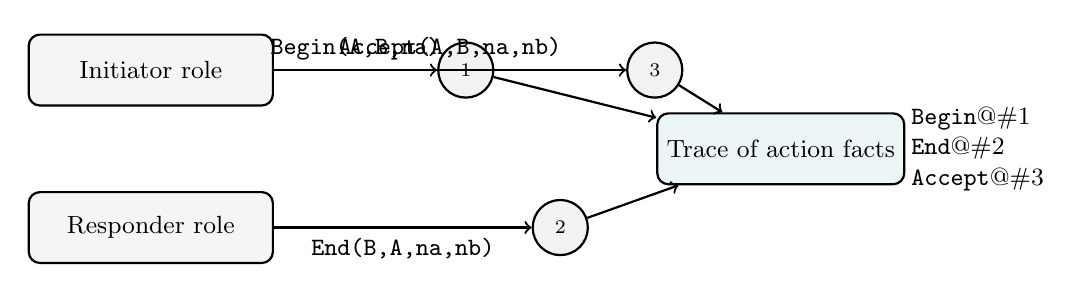
\begin{tikzpicture}[
      lane/.style={draw, rounded corners, minimum width=3.1cm,
                   minimum height=0.9cm, align=center, font=\small, thick},
      evt/.style={draw, circle, minimum size=7mm, font=\scriptsize, thick,
                  fill=gray!10},
      arr/.style={->, thick}
    ]
    \node[lane, fill=gray!8] (i) at (0,0) {Initiator role};
    \node[lane, fill=gray!8] (r) at (0,-2.0) {Responder role};
    \node[lane, fill=teal!8] (t) at (8,-1.0) {Trace of action facts};

    \node[evt] (e1) at (4,0) {$1$};
    \node[evt] (e2) at (5.2,-2.0) {$2$};
    \node[evt] (e3) at (6.4,0) {$3$};

    \draw[arr] (i) -- node[above, font=\small] {\texttt{Begin(A,B,na)}} (e1);
    \draw[arr] (r) -- node[below, font=\small] {\texttt{End(B,A,na,nb)}} (e2);
    \draw[arr] (i) -- node[above, font=\small] {\texttt{Accept(A,B,na,nb)}} (e3);

    \draw[arr] (e1) -- (t);
    \draw[arr] (e2) -- (t);
    \draw[arr] (e3) -- (t);
    \node[font=\small, align=left] at (10.5,-1.0)
      {$\texttt{Begin}@\#1$\\$\texttt{End}@\#2$\\$\texttt{Accept}@\#3$};
  \end{tikzpicture}
  \caption{A trace is the observable history of the run.  Action facts are
           attached to timepoints, which lets the logic express ordering and
           causality between protocol events.}
  \label{fig:tamarin-trace}
\end{figure}

\medskip\noindent
\textbf{Why traces are the right object.}  Security properties are rarely
about one isolated state.  They are about causality over time: a secret was
created before it was leaked; a responder accepted only after some initiator
really started; a key agreement happened only if both parties saw the same
fresh values.  The trace records exactly that causal history.

\subsection{A classical protocol pattern}

The Needham-Schroeder family of protocols is a classic teaching example for
Tamarin because it highlights the same ingredients in a slightly richer form:
fresh nonces, long-term keys, and correspondence between sends and receives.
One role starts with a fresh challenge, another role answers, and the
security question becomes whether the attacker can force a trace where the
answer is accepted without the expected prior event.

\medskip\noindent
The important lesson is not the exact message format.  It is the structure of
the specification:
\begin{enumerate}
  \item each honest role is described by a small number of rules;
  \item each important protocol step emits an action fact;
  \item the trace becomes the evidence for or against the security claim.
\end{enumerate}


% =======================================================================
\section{Equational Theories and Unification}
\label{sec:tamarin-unification}

In a free term algebra, two terms are equal if and only if they are syntactically identical. For example, the term $enc(m, k)$ and the variable $x$ do not match unless $x$ is bound to the exact syntax $enc(m, k)$.

However, real security protocols rely on cryptographic primitives where terms have algebraic relationships. For instance, decrypting a message with the correct key should yield the plaintext:
\[
  dec(enc(m, k), k) = m
\]
Here, the terms $dec(enc(m, k), k)$ and $m$ are syntactically different, but we want the system to treat them as semantically equivalent. To achieve this, Tamarin interprets terms modulo an \emph{equational theory} $E$ (a set of equations defining equivalence classes over terms).

\subsection{Semantic Equivalence in Attacker Knowledge}

The equational theory is the mechanism through which the Dolev-Yao attacker decrypts intercepted messages. Rather than deconstructing a term $enc(m, k)$ directly (which would violate the black-box assumption of ideal cryptography), the attacker operates by applying functions to terms they already know:
\begin{enumerate}
  \item The attacker intercepts $enc(m, k)$, learning the term: $\mathsf{K}(enc(m, k))$.
  \item Later, the attacker intercepts the key $k$, learning: $\mathsf{K}(k)$.
  \item Using the built-in term derivation rule, the attacker applies the decryption function symbol $dec$ to construct a new term:
  \[
    \mathsf{K}(dec(enc(m, k), k))
  \]
  \item Because the equational theory states that $dec(enc(m, k), k) \equiv_E m$, the term in the attacker's knowledge base is semantically equivalent to $m$. The attacker now knows the plaintext $m$.
\end{enumerate}

\subsection{The Unification Problem}

To apply a rewrite rule $L \xrightarrow{A} R$ to a concrete multiset of facts $M$, Tamarin must find a substitution $\sigma$ such that the facts in $L\sigma$ match a subset of $M$. This matching process requires solving equations between terms:
\begin{itemize}
  \item In the \emph{free term algebra} (syntactic equality), matching is a special case of unification. The classical \textbf{Martelli-Montanari} algorithm (1982) solves unification in linear time by repeatedly transforming equations into solved forms.
  \item Modulo an \emph{equational theory} $E$ ($E$-unification), we must find a substitution $\sigma$ such that $t_1\sigma \equiv_E t_2\sigma$. In full generality, $E$-unification is undecidable, and even when decidable, it can yield infinitely many minimal unifiers.
\end{itemize}

\subsection{Subterm-Convergent Theories}

To maintain decidability and efficiency, Tamarin permits the user to define custom equations, but restricts them to a class known as \textbf{subterm-convergent equational theories}. 

\begin{definition}[Subterm-Convergent Equation]
An equation $L = R$ is subterm-convergent if:
\begin{enumerate}
  \item It can be oriented as a rewrite rule $L \to R$ from left to right.
  \item The set of oriented rules is \emph{terminating} (there are no infinite chains of rewrites) and \emph{confluent} (rewriting a term in different orders always yields the same final result).
  \item The right-hand side $R$ is either a strict subterm of $L$ or a constant.
\end{enumerate}
\end{definition}

For example, $dec(enc(m, k), k) = m$ is subterm-convergent because the right-hand side $m$ is a subterm of the left-hand side. 

Because subterm-convergent equations simplify terms (reducing their size or complexity), they guarantee that any term can be rewritten to a unique, irreducible \emph{normal form} in linear time. Tamarin can then perform unification on these normal forms using the standard Martelli-Montanari style algorithm.

\subsection{Non-Subterm-Convergent Theories and Undecidability}

Many critical cryptographic primitives cannot be modeled with subterm-convergent equations. For example:
\begin{itemize}
  \item \textbf{Associativity}: $(x \cdot y) \cdot z = x \cdot (y \cdot z)$
  \item \textbf{Commutativity}: $x \cdot y = y \cdot x$
  \item \textbf{Diffie-Hellman exponentiation}: $(g^x)^y = (g^y)^x$
\end{itemize}
These equations do not reduce the size of terms and have no clear direction of simplification. If a user were to write $x \cdot y = y \cdot x$ as a rewriting rule, the engine would enter an infinite loop:
\[
  x \cdot y \;\longrightarrow\; y \cdot x \;\longrightarrow\; x \cdot y \;\longrightarrow\; \dots
\]
To handle these complex algebraic structures without sacrificing termination, Tamarin does not allow users to define arbitrary non-subterm-convergent equations. Instead, it provides built-in equational theories (such as \texttt{diffie-hellman}, \texttt{bilinear-pairing}, or \texttt{associative-commutative}) that are hard-coded into the core prover. These built-in theories use specialized algebraic unification algorithms that reason about equivalence classes directly rather than relying on naive term rewriting.

% =======================================================================
\section{Property Verification in Tamarin}
% Sources: Course 89, L28
\label{sec:tamarin-properties}

Once a protocol is written as rewrite rules, Tamarin checks properties stated
over traces.  The property language is a first-order logic whose variables
range over messages and timepoints.  That is enough to express the standard
verification questions in protocol analysis.

\begin{definition}[Trace formula]
\label{def:tamarin-formula}
A trace formula may quantify over terms and timepoints, refer to action facts
with the notation $F(t)@\#i$, and compare timepoints using relations such as
$\#i < \#j$.  Formulas are built from these atoms using the usual logical
connectives and quantifiers.
\end{definition}

\begin{intermezzo}{First-Order Logic Timepoints}
Why the strange \texttt{@\#i} notation? In standard First-Order Logic, to reason about an event occurring at a specific time, you would add a time parameter to a binary predicate, e.g., $\text{Event}(msg, t)$. Tamarin uses the \texttt{@} syntax to cleanly separate the protocol term (the message payload) from the temporal dimension (the trace index $\#i$). This separates the implicit timing of the rewriting rules from the explicit temporal logic of the properties.
\end{intermezzo}

The point of the logic is that it can state both local and temporal claims.
For example, a secrecy statement says that a message should never appear in
the intruder's knowledge; an authentication statement says that one event must
be preceded by another; and a reachability statement says that there exists a
trace satisfying a desired scenario.

\subsection{Secrecy}

Secrecy is the most basic property.  In Tamarin it is usually phrased as the
absence of intruder knowledge for a secret value.

\begin{example}[Secrecy lemma]
If \texttt{s} is a session secret, then a typical secrecy lemma has the form
\[
  \forall \#i.\ \mathsf{Secret}(s)@\#i \rightarrow \neg \exists \#j.\ \mathsf{K}(s)@\#j.
\]
The intended reading is: whenever the protocol marks a value as secret, the
attacker should never learn that value on any trace.
\end{example}

This is a good example of why traces matter.  The property is not asking
whether the secret is present in the current local state.  It is asking
whether the attacker can derive it at any point in the execution history.

\subsection{Authentication and correspondence}

Authentication is usually expressed as a correspondence between events.
One event claims that a participant has finished a session; another event
shows that the peer really started the same session earlier.

\begin{example}[Correspondence lemma]
Suppose a responder records \texttt{End(B,A,na,nb)} when it accepts a
session.  A standard agreement property says that every such acceptance must
have a prior initiator event:
\[
  \forall \#i.\ \mathsf{End}(B,A,na,nb)@\#i \rightarrow
  \exists \#j.\ \mathsf{Begin}(A,B,na)@\#j \land \#j < \#i.
\]
If the protocol is vulnerable to replay or impersonation, Tamarin will search
for a trace where \texttt{End} occurs without a matching earlier
\texttt{Begin}.  That trace is the attack witness.
\end{example}

The exact names of the action facts are up to the modeler.  What matters is
that the events are chosen to expose the security-relevant milestones of the
protocol.  Once those milestones are in place, the property reads like an
engineering statement about causality.

\subsection{Reachability and existence}

Not every property is universal.  Sometimes we want to know whether a desired
scenario is possible at all.  Tamarin supports existential trace queries for
that purpose.

\begin{example}[Existence of a good run]
If a protocol has a successful completion event \texttt{Done}, one may ask
whether there exists a trace that reaches it:
\[
  \exists \#i.\ \mathsf{Done}@\#i.
\]
This is useful during model construction.  Before proving that the protocol is
secure, we often first check that the model can actually execute the intended
good run.
\end{example}

\medskip\noindent
\textbf{What Tamarin returns.}  If the lemma is true, Tamarin produces a
proof.  If the lemma is false, it can return a counterexample trace showing an
attack.  If the search space is large, the proof may require user guidance in
the form of hints, induction, or careful lemma shaping.  The lecture point is
that the verification task is still trace-based: the prover is trying either
to establish a property of all traces or to expose one trace that violates it.

\begin{intermezzo}{How to read a Tamarin result}
The output is not just ``proved'' or ``failed''.  A good proof tells you that
all trace patterns allowed by the rules satisfy the lemma.  A counterexample
trace tells you exactly which sequence of rule applications breaks the claim.
That trace is usually the most valuable debugging artefact in the whole
analysis.
\end{intermezzo}

\subsection{Forward Secrecy}

A protocol that guarantees secrecy under normal runs might fail completely if long-term secrets are compromised in the future. For example, if an attacker records encrypted traffic today and steals the private key five years later, can they decrypt the old traffic? 

A protocol achieves \textbf{forward secrecy} (or perfect forward secrecy) if the compromise of long-term keys does not compromise past session keys.

To verify forward secrecy in Tamarin, we must explicitly model the capability of the attacker to compromise long-term keys. We do this by adding a \emph{key reveal rule} to our model:
\begin{lstlisting}
rule Reveal_Ltk:
  [ !Ltk(A, ltk) ]
  --[ Reveal(A) ]->
  [ Out(ltk) ]
\end{lstlisting}
This rule consumes the persistent long-term key fact $\mathsf{!Ltk}(A, ltk)$ and sends it on the network via $\mathsf{Out}$, which the Dolev-Yao attacker immediately learns. The action fact $\mathsf{Reveal}(A)$ is recorded on the trace to mark the exact moment of compromise.

We then write a forward secrecy lemma. It states that if a session key $K$ is established between Alice ($A$) and Bob ($B$) at timepoint $\#i$, the attacker can only learn $K$ if they compromised $A$ or $B$'s long-term key \emph{before} the session key was used:
\[
  \forall A, B, K, \#i.\ \mathsf{SessionKey}(A, B, K)@\#i \longrightarrow
  \left(
    \neg (\exists \#j.\ \mathsf{K}(K)@\#j) \;\lor\;
    (\exists \#r.\ \mathsf{Reveal}(A)@\#r \;\land\; \#r < \#i) \;\lor\;
    (\exists \#r.\ \mathsf{Reveal}(B)@\#r \;\land\; \#r < \#i)
  \right)
\]
If the attacker compromises a key at a future timepoint $\#r$ such that $\#i < \#r$, the formula requires that $\neg (\exists \#j.\ \mathsf{K}(K)@\#j)$ still holds. If Tamarin successfully proves this lemma, the protocol guarantees forward secrecy.

\subsection{Anonymity and Observational Equivalence}

Trace properties (like secrecy or agreement) are first-order formulas checked on individual traces. However, properties like \emph{anonymity}, \emph{privacy}, or \emph{untrackability} cannot be expressed as properties of a single trace. They are properties of the relations between different executions: can the attacker distinguish between two different system configurations?

To verify these properties, Tamarin uses \textbf{observational equivalence}. Instead of verifying a first-order logic formula on a trace, Tamarin checks if the attacker can distinguish between two slightly different processes.

In Tamarin, this is modeled by writing a single protocol specification that contains a special built-in function $\mathsf{diff}(x, y)$. This function instructs the compiler to generate two versions of the system:
\begin{itemize}
  \item System $L$, where the function evaluates to the left term $x$.
  \item System $R$, where the function evaluates to the right term $y$.
\end{itemize}
The prover then tries to show that for every execution in System $L$, there is a transition-by-transition equivalent execution in System $R$ that produces the exact same observable outputs to the attacker, and vice versa.

\begin{example}[Mobile Device Tracking and Anonymity in 5G]
Consider a mobile device $D$ that connects to multiple cell antennas as the user moves (a scenario critical to the 5G standard analysis mentioned earlier). We want to check whether an eavesdropper listening to the antenna traffic can track the user's location.
We set up a model where a device connects to Antenna 1 and then Antenna 2:
\begin{itemize}
  \item In System $L$, the same device ID $D$ connects to both antennas (simulating one user moving).
  \item In System $R$, device ID $D_1$ connects to Antenna 1, and a different device ID $D_2$ connects to Antenna 2 (simulating two different users).
\end{itemize}
We model this connection rule using the $\mathsf{diff}$ operator:
\begin{lstlisting}
rule Connect_Antenna_2:
  [ State_Device(D), In(request) ]
  -->
  [ Out(diff(D, D_prime)) ]
\end{lstlisting}
If Tamarin proves observational equivalence, it guarantees that the attacker cannot distinguish a single user moving between antennas from two distinct users. Thus, the protocol guarantees anonymity and untrackability. If the proof fails, Tamarin returns a counterexample showing how the attacker can track the device (e.g., because the device reused a static cookie, certificate, or unencrypted identifier).
\end{example}

\subsection{The modelling discipline}

Tamarin rewards disciplined models.  The rules should isolate the protocol
state you care about; action facts should mark the events you want to reason
about; and the properties should mention those events directly.  If the model
mixes too many concerns into one rule, the trace logic becomes hard to read.
If the action facts are too coarse, the proof loses the causal structure that
the property needs.  Good models are therefore not just correct; they are
observable.

This is the same engineering lesson that appeared in previous chapters in a
different guise: symbolic verification works best when the model separates
state, transition, and observation cleanly.  Tamarin just applies that lesson
to protocol histories.

% =======================================================================
\section{Summary}
% Sources: Course 89, L27-L28
\label{sec:tamarin-summary}

Tamarin verifies security protocols by turning them into multiset rewriting
systems and then reasoning about the traces those rules generate.  Terms model
symbolic messages.  Facts model local state, network events, and persistent
resources.  Protocol roles package rules into reusable participant templates.
Traces record the observable history of a run, and the property language
states secrecy, authentication, and reachability claims over those traces.

The chapter's main idea is that protocol verification is not graph checking in
the usual sense.  It is history checking.  Once that shift is clear, the rest
of the formalism becomes natural: fresh names explain new values, persistent
facts model long-term configuration, action facts expose relevant events, and
timepoints let the logic talk about order and causality.  That is the
Tamarin viewpoint in one sentence: specify the protocol as rewrite rules, and
specify the security claim as a property of the traces they produce.

\begin{summarybox}
\begin{itemize}[nosep]
  \item Security protocols are modelled as \emph{multiset rewriting systems}:
    terms represent symbolic messages, facts represent local and network
    state, and rules describe protocol steps.
  \item The \emph{Dolev--Yao attacker} controls the network: it can
    intercept, replay, and forge messages using any cryptographic
    operation whose key it knows.
  \item A \emph{trace} is the observable history of a protocol run;
    properties (secrecy, authentication, forward secrecy) are stated
    as first-order formulas over traces.
  \item \emph{Equational theories} capture algebraic properties of
    cryptographic primitives; subterm-convergent theories keep
    unification decidable.
  \item \emph{Tamarin} automates this pipeline: protocol rules in,
    proof or counterexample trace out.
\end{itemize}
\end{summarybox}

\section*{Exercises}
\addcontentsline{toc}{section}{Exercises}

\begin{chapex}[Dolev--Yao deduction]
The attacker knows the terms $\texttt{aenc}(m, \texttt{pk}(k))$ and $k$.
List the sequence of Dolev--Yao rules the attacker applies to recover
the plaintext~$m$.
\end{chapex}

\begin{chapex}[Trace reading]
A Tamarin trace contains the action facts
$\texttt{Secret}(m)$ at timepoint $\#i$ and
$\texttt{K}(m)$ at timepoint $\#j$ with $\#i < \#j$.
Does this trace satisfy the secrecy lemma
$\forall m,\,\#i.\;\texttt{Secret}(m)\mathbin{@}\#i \Rightarrow
  \neg(\exists\,\#j.\;\texttt{K}(m)\mathbin{@}\#j)$?
Explain your answer.
\end{chapex}

\begin{chapex}[Authentication encoding]
Write a Tamarin-style correspondence lemma expressing
\emph{non-injective agreement}: whenever Bob completes a session with
Alice on a shared key~$k$, Alice previously initiated a session with
the same~$k$.  Then explain what additional quantifier structure is
needed for \emph{injective} agreement.
\end{chapex}

\begin{chapex}[Forward secrecy]
Consider a protocol that uses a long-term key $\texttt{ltk}(A)$ to
encrypt a session key~$k_s$.  After the session, the attacker learns
$\texttt{ltk}(A)$.  Can the attacker recover $k_s$?  What protocol
mechanism would provide forward secrecy, and how would it change the
Tamarin model?
\end{chapex}
